\chapter{Orchestration-driven Service-oriented Architecture}

\section{Pendahuluan}

Orchestration-driven Service-oriented Architecture (SOA) merupakan pendekatan dalam pengembangan sistem terdistribusi yang menekankan pada pengelolaan alur proses bisnis melalui komponen pusat yang disebut orkestrator. Dalam arsitektur ini, orkestrator bertanggung jawab mengatur urutan eksekusi, pengambilan keputusan, serta koordinasi antar layanan secara eksplisit berdasarkan logika proses yang telah didefinisikan.

Berbeda dengan pendekatan \textit{choreography} yang bersifat desentralisasi, orkestrasi memberikan kontrol terpusat terhadap aliran proses, sehingga lebih mudah untuk dipantau, diuji, dan dimodifikasi. Layanan-layanan dalam SOA tetap bersifat loosely coupled dan reusable, namun interaksi antar layanan terjadi berdasarkan arahan dari orkestrator.

Arsitektur ini banyak digunakan dalam sistem enterprise dan integrasi lintas sistem, terutama pada skenario yang membutuhkan konsistensi transaksi, tracking proses, serta pengendalian alur kerja yang kompleks. Dengan memanfaatkan workflow engine seperti Camunda, Zeebe, atau Temporal, organisasi dapat merancang dan menjalankan proses bisnis secara modular, fleksibel, dan terotomatisasi, tanpa harus mengubah kode dari masing-masing layanan penyedia.

Pendekatan orkestrasi ini menjadi fondasi penting dalam membangun sistem informasi modern yang scalable, maintainable, dan selaras dengan kebutuhan bisnis yang terus berkembang.


\section{Konsep Dasar Orkestrasi Layanan}

\subsection{Definisi Orchestration dalam SOA}

Orchestration dalam konteks Service-oriented Architecture (SOA) merujuk pada pengelolaan dan pengendalian urutan eksekusi layanan-layanan terdistribusi oleh satu komponen pusat yang disebut \textit{orchestrator}. Orkestrasi mengatur bagaimana layanan saling berinteraksi dalam suatu workflow secara terkoordinasi dan terpusat, sehingga keseluruhan proses bisnis dapat dimodelkan, dijalankan, dan diawasi secara sistematis.

Orchestrator bertindak sebagai pengendali logika proses, mulai dari menentukan urutan layanan yang akan dipanggil, menangani input dan output dari setiap langkah, hingga mengatur bagaimana menangani kegagalan, melakukan retry, atau menginisiasi kompensasi. Pendekatan ini memberikan visibilitas penuh terhadap alur proses dan memungkinkan kontrol yang tinggi terhadap integrasi antar layanan dalam skenario bisnis kompleks.

\subsection{Perbedaan antara Orchestration dan Choreography}

Dalam SOA, dua pendekatan utama yang digunakan untuk mengatur interaksi layanan adalah orchestration dan choreography.

\begin{itemize}
	\item \textbf{Orchestration} bersifat \textit{terpusat}. Semua alur interaksi layanan dikendalikan oleh satu entitas pengatur (orchestrator) yang mengetahui dan mengarahkan setiap langkah dalam proses. Layanan yang terlibat tidak perlu mengetahui keseluruhan proses, cukup menanggapi permintaan dari orchestrator.
	
	\item \textbf{Choreography} bersifat \textit{terdistribusi}. Tidak ada satu entitas pengendali pusat; setiap layanan mengetahui kapan harus berinteraksi dengan layanan lain dan bertindak sesuai peran masing-masing dalam proses. Komunikasi terjadi secara peer-to-peer berdasarkan aturan (rules) yang telah disepakati.
\end{itemize}

Perbedaan utamanya terletak pada kontrol dan visibilitas. Orchestration memberikan kontrol lebih kuat dan kemudahan pengelolaan proses secara end-to-end, namun menimbulkan ketergantungan pada orchestrator. Sementara itu, choreography menawarkan skalabilitas dan desentralisasi yang lebih baik, tetapi sulit dikelola pada sistem dengan alur bisnis kompleks.

\subsection{Komponen Utama dalam Orchestration}

Beberapa komponen penting dalam implementasi arsitektur orkestrasi layanan meliputi:

\begin{enumerate}
	\item \textbf{Orchestrator Engine} \\
	Komponen inti yang menjalankan workflow berdasarkan definisi proses bisnis. Engine ini bertanggung jawab mengatur alur eksekusi, melakukan pemanggilan layanan, menangani keputusan bercabang, serta mencatat status proses. Contoh orchestrator engine termasuk Camunda, Zeebe, Temporal, dan Apache ODE.
	
	\item \textbf{Process Definition (Workflow)} \\
	Deskripsi formal dari urutan langkah dalam proses bisnis, biasanya ditulis menggunakan BPMN (Business Process Model and Notation) atau DSL (Domain-Specific Language) tertentu. Definisi ini berisi aktivitas, urutan, kondisi, serta aturan eksekusi antar layanan.
	
	\item \textbf{Service Tasks} \\
	Unit eksekusi dalam workflow yang merepresentasikan pemanggilan ke layanan eksternal. Setiap service task dihubungkan ke endpoint API tertentu dan dapat dikonfigurasi untuk menangani input/output serta error.
	
	\item \textbf{Data Mapping dan Transformation} \\
	Mekanisme untuk mengubah atau memformat data antar langkah dalam workflow agar sesuai dengan spesifikasi masing-masing layanan. Orchestrator biasanya menyediakan fitur mapping input/output dan ekspresi transformasi data.
	
	\item \textbf{Monitoring dan Audit Trail} \\
	Fasilitas untuk memantau eksekusi proses, melacak status task, menganalisis kegagalan, serta menghasilkan jejak audit yang berguna untuk debugging, compliance, dan pelaporan.
	
	\item \textbf{Error Handling dan Compensation} \\
	Strategi penanganan kegagalan, seperti retry otomatis, branching ke jalur alternatif, dan pengaktifan aktivitas kompensasi untuk membatalkan efek dari langkah-langkah sebelumnya jika terjadi kesalahan dalam proses.
\end{enumerate}


\section{Contoh Kasus Penggunaan}

\subsection{Sistem Pemesanan Tiket Multi-Layanan}

Salah satu contoh nyata implementasi Orchestration-driven SOA adalah pada sistem pemesanan tiket yang melibatkan beberapa layanan eksternal, seperti layanan penerbangan, hotel, transportasi darat, dan pembayaran. Dalam kasus ini, orchestrator mengelola urutan pemesanan agar seluruh proses berjalan konsisten dan atomik.

Sebagai contoh, ketika pengguna memesan tiket paket liburan melalui aplikasi, orchestrator akan mengatur alur sebagai berikut: pertama memanggil layanan penerbangan untuk mencari ketersediaan tiket, kemudian layanan hotel untuk reservasi kamar, diikuti oleh pemesanan transportasi lokal, dan terakhir layanan pembayaran. Jika salah satu langkah gagal (misalnya hotel tidak tersedia), orchestrator akan menjalankan proses kompensasi, seperti membatalkan tiket pesawat yang sudah dipesan.

Pendekatan ini memastikan koordinasi penuh antar layanan, menjaga integritas data pemesanan, dan menyediakan audit trail yang jelas terhadap seluruh proses pemesanan.

\subsection{Automasi Proses Bisnis di Perusahaan Jasa}

Di perusahaan jasa seperti asuransi, leasing, atau logistik, banyak proses bisnis bersifat berulang dan membutuhkan interaksi antar banyak sistem. Contoh proses seperti pengajuan klaim asuransi, permintaan layanan pelanggan, atau proses onboarding mitra dapat diotomatisasi menggunakan orkestrasi.

Misalnya, dalam pengajuan klaim asuransi kendaraan, orchestrator mengatur langkah-langkah seperti: menerima formulir pengajuan, memvalidasi dokumen melalui OCR service, memverifikasi data kendaraan dengan sistem registrasi nasional, menghitung estimasi kerusakan melalui layanan pihak ketiga, dan akhirnya memicu pembayaran klaim jika klaim disetujui.

Dengan orkestrasi, proses tersebut dapat dimodelkan secara visual, dijalankan secara otomatis, serta dimonitor oleh staf untuk intervensi manual jika diperlukan. Hal ini meningkatkan efisiensi operasional, mengurangi waktu penyelesaian, dan menghindari duplikasi kerja antar divisi.

\subsection{Integrasi Antar Aplikasi di Lingkungan Enterprise}

Dalam lingkungan enterprise yang kompleks, aplikasi-aplikasi sering dikembangkan oleh tim yang berbeda dan beroperasi pada platform yang beragam. Orkestrasi memungkinkan integrasi antar aplikasi tersebut tanpa perlu membuat perubahan besar pada masing-masing sistem.

Contohnya adalah integrasi antara sistem HR, payroll, dan sistem keuangan. Ketika seorang karyawan baru direkrut, orchestrator dapat secara otomatis:
\begin{enumerate}
	\item Menambahkan data karyawan ke sistem HR.
	\item Membuat akun gaji dan menghitung pro-rata salary di sistem payroll.
	\item Mengalokasikan anggaran pelatihan awal di sistem keuangan.
	\item Mengirim notifikasi ke manajer dan staf terkait untuk approval dan koordinasi.
\end{enumerate}

Tanpa orkestrasi, integrasi semacam ini akan bergantung pada skrip ad-hoc atau komunikasi manual antar sistem. Dengan orkestrator, seluruh proses menjadi transparan, terdokumentasi, dan lebih mudah diatur ulang jika terjadi perubahan bisnis atau regulasi.


\section{Kelebihan dan Kekurangan}

\subsection{Kelebihan}
Penerapan arsitektur Orchestration-driven Service-oriented Architecture (SOA) memberikan berbagai keunggulan yang signifikan, khususnya dalam sistem berskala besar yang membutuhkan koordinasi layanan yang kompleks dan terdistribusi. Salah satu kelebihan utama dari pendekatan ini adalah kemampuannya dalam mengelola proses bisnis secara terpusat dan eksplisit. Dengan menggunakan orchestrator, organisasi dapat dengan mudah memodelkan alur proses dalam bentuk workflow yang terstruktur, memantau status eksekusinya secara real-time, serta melakukan tracing atas setiap interaksi antar layanan yang terlibat.

Selain itu, arsitektur orkestrasi memudahkan adaptasi terhadap perubahan bisnis. Jika terjadi perubahan dalam aturan proses, orchestrator cukup diperbarui tanpa harus mengubah kode masing-masing layanan yang terlibat. Hal ini memberikan fleksibilitas tinggi, terutama dalam organisasi yang menghadapi dinamika regulasi atau kebutuhan pelanggan yang terus berkembang. Dengan pendekatan modular yang terintegrasi melalui orchestrator, pengujian proses bisnis juga menjadi lebih terukur karena dapat dilakukan secara isolasi terhadap definisi workflow.

Dari sisi efisiensi pengembangan dan kolaborasi tim, orchestrasi mendukung pemisahan tanggung jawab secara jelas antara tim bisnis dan tim teknis. Tim bisnis dapat terlibat langsung dalam merancang logika proses menggunakan notasi visual seperti BPMN, sementara tim teknis fokus pada pengembangan layanan-layanan spesifik yang dihubungkan melalui workflow. Ini mempercepat siklus pengembangan dan memfasilitasi komunikasi lintas peran.

\subsection{Kekurangan}
Namun demikian, pendekatan orkestrasi juga memiliki keterbatasan yang perlu diperhatikan. Salah satu tantangan utamanya adalah meningkatnya ketergantungan terhadap orchestrator sebagai komponen pusat. Kegagalan atau bottleneck pada orchestrator dapat berdampak luas terhadap keseluruhan proses bisnis. Oleh karena itu, penerapan orchestrator harus dirancang dengan redundansi dan pengawasan ketat.

Selain itu, orkestrasi dapat menimbulkan kompleksitas tambahan dalam hal debugging dan monitoring jika tidak dilengkapi dengan sistem observabilitas yang memadai. Karena proses berjalan lintas banyak layanan dan sering kali melibatkan komunikasi asinkron, tracing dan root cause analysis menjadi lebih sulit tanpa dukungan alat seperti distributed tracing dan centralized logging.

Kelemahan lain yang perlu dipertimbangkan adalah potensi overhead kinerja karena orchestrator harus terus mengelola status dan dependensi antar langkah. Dalam beban kerja yang sangat tinggi, orchestrator yang tidak dioptimalkan dapat menjadi titik lemah sistem. Dalam konteks ini, pendekatan choreography yang lebih ringan dan terdistribusi dapat menjadi alternatif, meskipun dengan tantangan koordinasi yang berbeda.

Secara keseluruhan, arsitektur berbasis orkestrasi sangat sesuai untuk organisasi yang membutuhkan kontrol alur proses yang kuat, konsistensi eksekusi, dan visibilitas lintas sistem. Namun keberhasilannya sangat bergantung pada kualitas desain workflow, pemilihan teknologi orchestrator yang tepat, serta kesiapan infrastruktur dan tim dalam mengelola kompleksitas sistem yang terpusat.


\section{Arsitektur dan Desain Sistem}

\begin{figure}
	\centering
	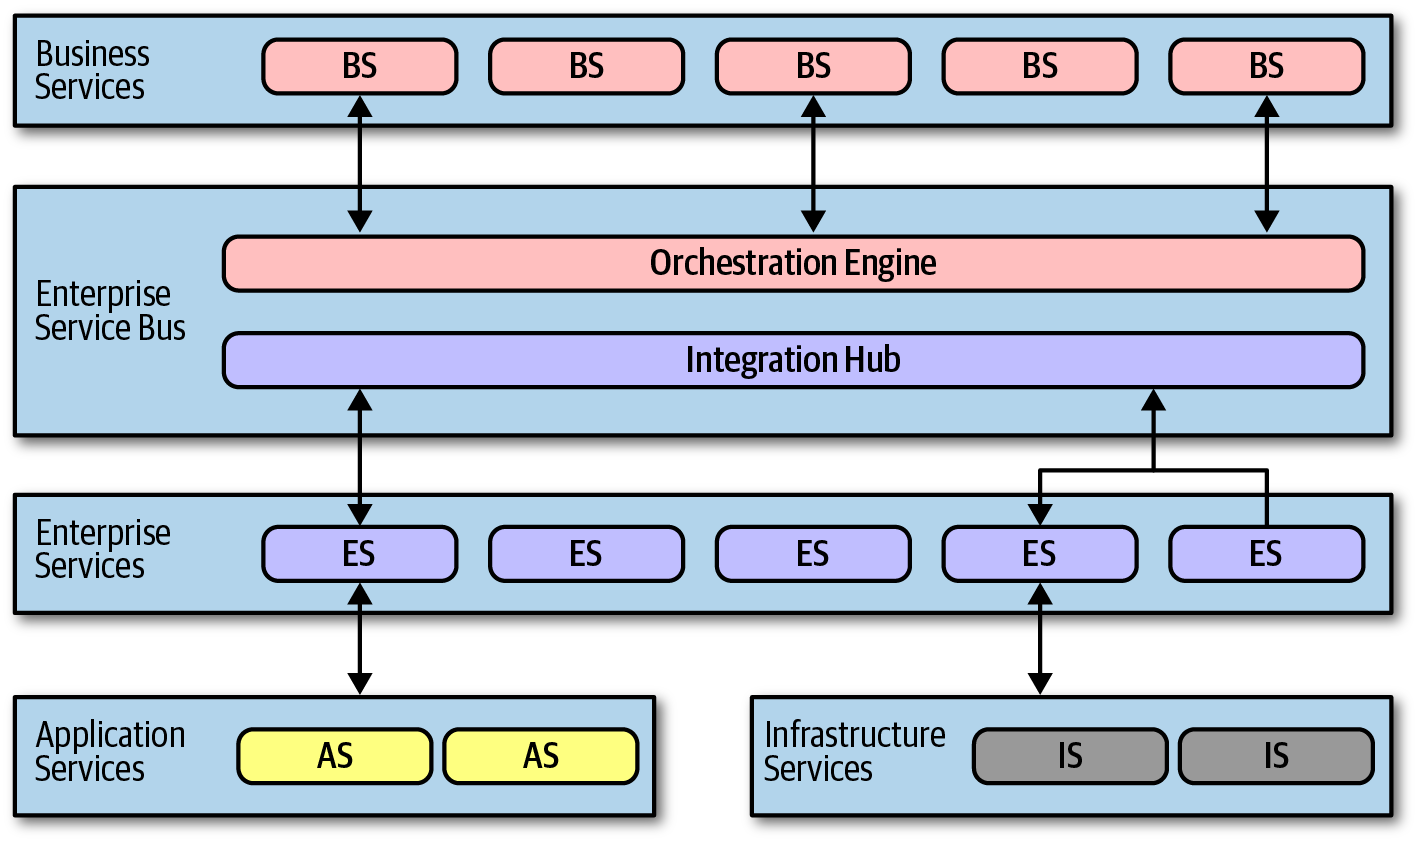
\includegraphics[width=\textwidth]{../images/orchestration-example}
\end{figure}
Dalam implementasi Orchestration-driven Service-oriented Architecture (SOA), sistem dibangun secara modular dan berlapis, memisahkan tanggung jawab setiap komponen berdasarkan perannya dalam mendukung proses bisnis secara menyeluruh. Pendekatan ini mempermudah integrasi, skalabilitas, pengelolaan dependensi, serta pengendalian alur proses bisnis yang kompleks. Berikut adalah komponen utama dalam arsitektur sistem orkestrasi layanan:

\subsection{Business Services}
Business Services merupakan representasi logika bisnis tingkat tinggi yang merepresentasikan proses-proses utama dalam organisasi, seperti pemesanan, klaim, penggajian, atau pengelolaan pelanggan. Layanan ini tidak berdiri sebagai satu unit tunggal, tetapi merupakan komposisi dari sejumlah layanan aplikasi (application services) yang dikendalikan melalui proses orkestrasi.

Sebagai contoh, dalam sistem pemesanan paket perjalanan, business service \textit{BookTravelPackage} dapat mencakup serangkaian langkah seperti pemesanan tiket pesawat, reservasi hotel, penyediaan transportasi lokal, dan pencatatan data pelanggan. Semua langkah tersebut dijalankan oleh layanan yang berbeda, namun dikoordinasikan oleh satu workflow yang dieksekusi oleh orchestrator. Workflow ini biasanya didefinisikan dalam bentuk BPMN (Business Process Model and Notation) dan dijalankan menggunakan engine seperti Camunda.

Secara teknis, business service direpresentasikan dalam bentuk definisi proses berbasis BPMN, YAML, atau DSL tertentu yang kemudian dideploy ke workflow engine. Engine seperti Camunda BPM menyediakan lingkungan berbasis Java dengan dukungan penuh terhadap BPMN 2.0. Zeebe, yang dikembangkan oleh tim Camunda, menawarkan workflow engine berbasis event dengan skalabilitas tinggi untuk microservices. Temporal, yang mendukung bahasa Go dan Java, digunakan untuk membangun workflow yang tahan terhadap gangguan (durable execution). Di bidang data engineering, Apache Airflow sering digunakan untuk mengelola workflow batch, meskipun kurang cocok untuk orkestrasi proses bisnis real-time.

Business Services sangat penting karena menyediakan visibilitas penuh terhadap proses lintas sistem, serta memungkinkan adaptasi cepat terhadap perubahan proses bisnis tanpa mengubah kode layanan di bawahnya.

\subsection{Enterprise Service Bus}
Enterprise Service Bus (ESB) adalah komponen middleware yang memfasilitasi komunikasi antar layanan dan sistem secara terstandar, terstruktur, dan terintegrasi. Fungsinya mencakup pengiriman pesan, transformasi format data (misalnya dari XML ke JSON), routing ke layanan tujuan, serta pengelolaan protokol dan keamanan komunikasi. Selain itu, ESB juga memungkinkan penerapan aturan bisnis, logging, dan monitoring trafik antar layanan.

Sebagai ilustrasi, dalam sistem keuangan yang perlu mengirimkan data transaksi ke sistem pelaporan dan sistem audit secara paralel, ESB dapat bertindak sebagai perantara yang menggandakan pesan, mengonversi data ke format yang sesuai dengan masing-masing sistem, dan mengatur antrian agar sistem downstream tidak kelebihan beban.

Teknologi yang umum digunakan untuk membangun ESB antara lain Apache ServiceMix dan Mule ESB yang berbasis Java dan mendukung integrasi standar industri. WSO2 Enterprise Integrator juga sering digunakan karena menyediakan fitur orkestrasi layanan, mediasi, serta pemetaan data. Untuk kebutuhan enterprise yang lebih kompleks, Red Hat Fuse (sebelumnya JBoss Fuse) menyediakan lingkungan pengembangan berbasis Apache Camel yang mendukung routing dinamis dan transformasi pesan. Bagi pengembang yang memilih pendekatan ringan, Spring Integration atau Apache Camel dapat digunakan sebagai basis ESB modular tanpa platform berat.

Meskipun demikian, pada arsitektur modern berbasis event, banyak fungsi tradisional ESB kini digantikan oleh kombinasi event broker seperti Apache Kafka, service mesh seperti Istio, serta orkestrator desentralistik. Namun ESB tetap relevan di lingkungan enterprise yang masih banyak bergantung pada integrasi sistem warisan (legacy system) dan komunikasi sinkron.


\subsection{Orchestration Engine}
 Orchestration Engine adalah inti dari sistem yang bertanggung jawab menjalankan workflow proses bisnis secara terstruktur. Engine ini berperan sebagai pengendali utama yang menentukan urutan eksekusi layanan, menangani aliran data antar tahapan, memantau status eksekusi tiap langkah, dan merespons event serta kesalahan yang terjadi selama proses berlangsung. Engine bekerja berdasarkan definisi proses bisnis yang ditulis dalam format standar seperti BPMN (Business Process Model and Notation) atau DSL (Domain Specific Language) tertentu.

Dalam praktiknya, orchestrator akan mengeksekusi proses secara sinkron maupun asinkron, tergantung pada jenis layanan yang dipanggil. Misalnya, dalam skenario pemrosesan order pelanggan, orchestrator akan mengeksekusi langkah-langkah seperti validasi data, pengecekan stok barang, penghitungan total harga, dan pemanggilan sistem pembayaran secara berurutan. Setiap langkah tersebut dapat dikonfigurasi untuk mengakses API tertentu, memproses response, dan memicu langkah berikutnya. Jika terjadi error, orchestrator dapat menjalankan mekanisme retry otomatis, percabangan ke jalur alternatif, atau menjalankan kompensasi.

Beberapa teknologi populer yang digunakan sebagai orchestration engine meliputi Camunda BPM, Zeebe, dan Temporal. Camunda BPM mendukung definisi proses berbasis BPMN 2.0 dan banyak digunakan dalam sistem enterprise berbasis Java. Zeebe, sebagai generasi baru dari Camunda, dirancang untuk kebutuhan event-driven dan microservices dengan skalabilitas tinggi. Sementara itu, Temporal adalah workflow engine berbasis kode (code-first) yang banyak digunakan dalam ekosistem cloud-native karena mendukung durabilitas, retries otomatis, dan kompensasi melalui bahasa pemrograman seperti Go dan Java.

Keberadaan orchestration engine memberikan keunggulan dalam hal observabilitas, kemampuan tracing proses end-to-end, serta fleksibilitas dalam mengubah alur proses tanpa harus memodifikasi layanan-layanan individual yang terlibat.

\subsection{Integration Hub}.
 Integration Hub merupakan komponen yang menjembatani integrasi antar sistem atau layanan yang memiliki format data, protokol komunikasi, dan kebutuhan autentikasi yang berbeda. Dalam lingkungan enterprise, aplikasi-aplikasi yang digunakan seringkali dibangun oleh tim berbeda, berasal dari generasi teknologi berbeda, atau bahkan dimiliki oleh pihak ketiga. Integration Hub memungkinkan sistem-sistem tersebut tetap dapat berkomunikasi secara lancar dengan menyediakan lapisan abstraksi yang menyatukan perbedaan teknis antar aplikasi.

Fungsi utama dari Integration Hub mencakup normalisasi data, transformasi format (misalnya dari XML ke JSON atau sebaliknya), pengaturan rute pesan berdasarkan isi (content-based routing), penjadwalan pemrosesan data, serta penyisipan logika tambahan seperti validasi atau pengayaan (enrichment) data sebelum diteruskan ke sistem tujuan. Sebagai contoh, ketika data pelanggan dikirim dari sistem CRM ke sistem keuangan, Integration Hub dapat melakukan pemetaan ulang struktur data, menambahkan metadata tambahan seperti timestamp, dan mengubah protokol dari REST ke SOAP.

Secara teknis, Integration Hub dapat dibangun menggunakan platform integrasi seperti WSO2 Enterprise Integrator yang menyediakan mediasi dan transformasi data melalui konfigurasi visual maupun skrip, atau melalui Apache Camel yang memungkinkan developer menulis rute dan logika transformasi dalam bahasa Java atau XML. Dalam pendekatan yang lebih ringan dan modern, pengembang dapat memanfaatkan middleware berbasis event seperti Apache Kafka bersama Kafka Connect untuk integrasi berbasis streaming data, atau menggunakan cloud-native tools seperti AWS EventBridge atau Azure Logic Apps untuk integrasi lintas layanan dengan sedikit kode.

Integration Hub tidak hanya memudahkan integrasi, tetapi juga memperkuat aspek keamanan dan monitoring karena seluruh lalu lintas antar sistem dapat dipusatkan, dipantau, dan dikelola dari satu titik. Ini sangat penting untuk memastikan auditabilitas, troubleshooting, dan pengendalian akses pada sistem yang terdistribusi.


\subsection{Enterprise Services}. 
Enterprise Services adalah layanan-layanan reusable yang mewakili perilaku atomik dari suatu domain bisnis tertentu, seperti \textit{VerifyIdentity}, \textit{CalculateCreditScore}, atau \textit{GenerateContract}. Layanan ini dikembangkan dengan tingkat granularitas yang cukup kecil agar dapat digunakan kembali dalam berbagai alur proses bisnis dan business services yang berbeda, sekaligus cukup bermakna agar tidak terlalu teknis seperti application services murni. Enterprise services bersifat fine-grained, dan berfungsi sebagai blok penyusun (building blocks) bagi orchestrator dalam membentuk layanan bisnis yang lebih besar.

Sebagai contoh, \textit{EvaluateCreditworthinessService} dapat digunakan dalam business service untuk pengajuan pinjaman, pembukaan rekening baru, maupun approval limit kartu kredit. Demikian pula, \textit{GenerateDigitalContractService} dapat digunakan tidak hanya dalam proses pinjaman, tetapi juga dalam business service seperti e-signing kontrak kerja sama vendor. Karena reusable, enterprise services dikembangkan dengan standar API yang stabil, terdokumentasi, dan diisolasi dari sistem tertentu. Mereka biasanya hanya fokus pada satu tanggung jawab logis dan tidak tergantung pada antarmuka pengguna atau platform penyimpanan tertentu.

Secara teknis, enterprise services dapat diimplementasikan dengan memanfaatkan satu atau lebih application services di bawahnya. Misalnya, enterprise service untuk verifikasi identitas mungkin memanggil application service untuk melakukan OCR dokumen dan pemeriksaan database kependudukan. Meskipun begitu, enterprise services tetap menjaga antarmuka logika bisnis yang bersih agar dapat digunakan oleh berbagai business service tanpa bergantung pada platform atau teknologi implementasinya.

\subsection{Application Services}. 
Application Services adalah layanan yang menyediakan fungsi-fungsi teknis spesifik dari suatu aplikasi atau sistem tertentu. Layanan ini biasanya terikat pada konteks platform atau unit sistem individual, dan tidak dirancang untuk digunakan secara lintas domain bisnis. Application services bisa berupa layanan yang melakukan ekstraksi data dari sistem monolitik, melakukan OCR pada gambar dokumen, menjalankan model machine learning, atau menghasilkan file PDF berdasarkan template.

Berbeda dengan enterprise services yang mendefinisikan makna bisnis secara atomik, application services lebih dekat ke pelaksanaan teknis dari suatu tugas. Misalnya, \textit{OCRApplicationService}, \textit{MLScoringService}, dan \textit{PDFGenerationService} masing-masing melakukan satu tugas spesifik yang kemudian dikombinasikan oleh enterprise service untuk membentuk perilaku bisnis yang utuh.

Application services dapat berupa microservices, library internal, atau wrapper terhadap sistem lama (legacy). Mereka sering kali hanya digunakan dalam konteks tertentu—misalnya hanya untuk modul verifikasi KYC atau untuk sistem helpdesk internal. Dalam arsitektur orkestrasi, application services tidak dipanggil langsung oleh orchestrator, melainkan dipanggil oleh enterprise services yang menyatukan fungsionalitasnya menjadi satu API bisnis yang koheren.

Application services idealnya dirancang dengan prinsip single responsibility, idempoten, dan memiliki observabilitas yang baik. Mereka juga harus cukup fleksibel untuk digunakan oleh berbagai enterprise service jika dibutuhkan, meskipun cakupan pemakaiannya biasanya lebih terbatas.


\subsection{Infrastructure Services}. 
Infrastructure Services merupakan lapisan dukungan teknis yang menyediakan fungsionalitas-fungsionalitas fundamental yang digunakan oleh berbagai komponen lain dalam arsitektur. Layanan ini bersifat reusable, tidak spesifik terhadap domain bisnis tertentu, dan biasanya dikelola oleh tim DevOps, SRE, atau platform engineering. Infrastruktur ini menjadi tulang punggung dari sistem orkestrasi karena mendukung operasional, komunikasi, dan observabilitas dari seluruh workflow dan layanan yang terlibat.

Contoh paling umum dari infrastructure services adalah layanan penyimpanan data, seperti database relasional (PostgreSQL, MySQL), database NoSQL (MongoDB, DynamoDB), atau object storage seperti Amazon S3 dan Google Cloud Storage. Untuk komunikasi antar layanan, sistem messaging seperti Apache Kafka, RabbitMQ, atau AWS SNS/SQS digunakan untuk membangun pola komunikasi event-driven. Selain itu, sistem monitoring dan observabilitas seperti Prometheus untuk metrik, ELK stack untuk log sentral, dan Grafana untuk visualisasi sangat penting dalam mendukung pengawasan dan debugging sistem orkestrasi.

Dalam arsitektur modern, service discovery (seperti Consul atau Eureka), configuration management (seperti Spring Cloud Config atau HashiCorp Vault), serta container orchestration (seperti Kubernetes) juga termasuk ke dalam lapisan infrastructure services. Semua komponen ini bekerja secara horizontal mendukung seluruh aplikasi tanpa perlu memahami logika bisnis secara langsung. Ketahanan, skalabilitas, dan latensi dari layanan-layanan infrastruktur ini memiliki dampak besar terhadap stabilitas keseluruhan proses orkestrasi. Oleh karena itu, pemantauan yang aktif, strategi failover, dan pengujian beban berkala menjadi bagian penting dari operasionalisasi infrastructure services.


\subsection*{Contoh Implementasi: Skenario Pengajuan Pinjaman Digital}

Seorang pengguna bernama Andi membuka aplikasi pinjaman digital dan mengisi formulir pengajuan. Saat ia menekan tombol “Ajukan Pinjaman”, sistem mengaktifkan \textbf{Business Service} utama bernama \textit{LoanApplicationProcessing}. Business service ini didefinisikan dalam bentuk workflow BPMN yang mengatur urutan langkah proses bisnis seperti validasi identitas, analisis kelayakan kredit, pembuatan kontrak digital, pencairan dana, dan pengiriman notifikasi. Business service tidak menjalankan langkah-langkah ini secara langsung, melainkan mengoordinasikan sejumlah layanan di bawahnya melalui orchestrator.

Langkah-langkah dalam business service ini dijalankan oleh kombinasi antara \textbf{Enterprise Services} dan \textbf{Application Services}. Sebagai contoh, \textit{VerifyIdentityService}, \textit{EvaluateCreditworthinessService}, dan \textit{GenerateContractService} adalah \textbf{Enterprise Services} karena mereka bersifat fine-grained, reusable, dan dapat digunakan kembali dalam konteks proses bisnis lain seperti pembukaan rekening atau perpanjangan pinjaman. Layanan-layanan ini mewakili logika bisnis atomik dan dikembangkan agar dapat digunakan lintas modul melalui kontrak API yang stabil.

Di sisi lain, untuk melakukan operasi teknis seperti OCR terhadap dokumen KTP, memanggil model machine learning untuk prediksi risiko, atau membuat file PDF untuk kontrak, masing-masing enterprise service ini akan memanggil \textbf{Application Services} yang lebih spesifik dan terikat pada teknologi atau platform tertentu. Misalnya, `VerifyIdentityService` memanggil `OCRApplicationService`, `EvaluateCreditworthinessService` memanggil `MLScoringService`, dan `GenerateContractService` menggunakan `PDFGeneratorService`. Application services biasanya memiliki fungsi tertentu, seperti generate pdf, machine learning analytics, kirim email, komunikasi dengan aplikasi eksternal, dsb.

Untuk komunikasi dan koordinasi antara layanan-layanan tersebut, data ditransmisikan antar sistem menggunakan \textbf{Enterprise Service Bus (ESB)}. ESB menangani transformasi format data (misalnya dari JSON ke XML), mengelola koneksi ke sistem eksternal seperti SLIK OJK, serta mendistribusikan hasil pemrosesan ke sistem pelaporan dan audit. Routing dan keamanan komunikasi juga diatur secara terpusat melalui ESB. ESB terdiri dari 2 komponen, yaitu Orchestration Engine dan Integration Hub.

Seluruh alur proses dikoordinasikan oleh \textbf{Orchestration Engine} seperti Camunda BPM. Engine ini menjalankan workflow bisnis secara terstruktur, mengelola status setiap langkah, dan menangani event atau error seperti retry atau kompensasi bila terjadi kegagalan pada salah satu layanan. Branching logika juga dapat diatur, misalnya jika pinjaman melebihi nominal tertentu, orchestrator memicu jalur approval manual.

Agar integrasi antar sistem dapat dilakukan dengan lancar, \textbf{Integration Hub} digunakan untuk menjembatani komunikasi antara sistem CRM, sistem pelanggan lama, dan enterprise services. Integration hub seperti Apache Camel melakukan normalisasi struktur data, enrich metadata, dan transformasi protokol komunikasi antar sistem.

\textbf{Infrastructure Services} menjadi fondasi teknis dari seluruh sistem ini. Data disimpan dalam PostgreSQL dan MongoDB, sementara cache digunakan melalui Redis. Komunikasi asynchronous didukung oleh Apache Kafka. Monitoring dilakukan menggunakan Prometheus dan Grafana, sedangkan log dan tracing dikumpulkan melalui ELK Stack dan OpenTelemetry. Semua komponen dijalankan di atas Kubernetes dengan manajemen konfigurasi melalui Spring Cloud Config dan service discovery menggunakan Consul.

Dengan pemisahan yang jelas antara enterprise services dan application services, arsitektur ini memungkinkan pengembangan sistem yang modular dan scalable. Enterprise services dapat digunakan ulang dalam berbagai business service lain, sementara application services memberikan dukungan teknis spesifik terhadap kebutuhan implementasi dari layanan-layanan tersebut. Dengan orchestrator sebagai pengendali utama, sistem ini memberikan fleksibilitas dan visibilitas penuh terhadap proses bisnis yang kompleks seperti pengajuan pinjaman digital.


\section{Pola Implementasi}

Pola implementasi dalam Orchestration-driven Service-oriented Architecture sangat menentukan bagaimana orkestrasi dijalankan secara operasional, bagaimana layanan berinteraksi, serta bagaimana sistem dirancang untuk mendukung konsistensi, skalabilitas, dan observabilitas. Terdapat beberapa pendekatan umum yang sering diterapkan dalam dunia nyata untuk merealisasikan orkestrasi secara efektif.

\subsection{Centralized Orchestrator}

Pola ini menempatkan satu komponen utama—disebut orchestrator—sebagai pengendali pusat alur proses bisnis. Orchestrator bertanggung jawab terhadap urutan eksekusi, penanganan error, kontrol alur bercabang, serta pelacakan status proses end-to-end. Dalam pendekatan ini, seluruh layanan yang terlibat bertindak sebagai "aktor pasif" yang menunggu instruksi dari orchestrator, dan tidak mengetahui keseluruhan konteks proses.

Contoh klasik penerapan centralized orchestrator dapat ditemukan dalam sistem pemrosesan order e-commerce, di mana orchestrator mengatur alur dari mulai validasi order, pengecekan stok, pembuatan invoice, hingga konfirmasi pembayaran. Camunda BPM dan Temporal adalah dua teknologi populer yang mendukung pendekatan ini. Meskipun pola ini memberikan visibilitas dan kendali tinggi, ia juga membawa tantangan dalam hal skalabilitas dan ketahanan (resilience), karena orchestrator menjadi komponen sentral yang harus dijaga keandalannya secara khusus.

\subsection{Orchestrated Microservices}

Dalam konteks arsitektur microservices, orchestrasi digunakan untuk mengatur koordinasi antar layanan-layanan kecil yang memiliki tanggung jawab spesifik. Meskipun masing-masing microservice dapat berjalan secara independen, orchestrator digunakan untuk menyatukan layanan-layanan tersebut ke dalam suatu alur kerja yang kompleks.

Misalnya, dalam sistem manajemen pengiriman barang, terdapat layanan terpisah untuk manajemen inventori, logistik, pelacakan GPS, dan notifikasi pelanggan. Orchestrator memanggil masing-masing layanan ini sesuai urutan logika bisnis: setelah barang dikemas oleh layanan logistik, orchestrator memicu layanan pelacakan untuk memulai monitoring lokasi, lalu mengaktifkan layanan notifikasi untuk memberi tahu pelanggan. Pendekatan ini memungkinkan pengembangan yang terdistribusi oleh tim berbeda, tetapi tetap menjaga keselarasan dalam proses bisnis secara keseluruhan.

Keberhasilan orchestrated microservices sangat dipengaruhi oleh kejelasan kontrak layanan, idempotensi fungsi, dan standar komunikasi seperti REST atau gRPC. Kombinasi orchestrator seperti Zeebe dengan protokol komunikasi yang ringan menjadikan pola ini fleksibel dan cocok untuk cloud-native deployment.

\subsection{Long-running Business Transactions (Saga dalam SOA)}

Tidak semua proses bisnis dapat diselesaikan dalam satu kali eksekusi cepat. Dalam sistem keuangan, supply chain, atau pelayanan publik, sering kali transaksi berlangsung dalam waktu yang panjang dan melibatkan beberapa sistem yang saling bergantung. Pola Saga digunakan untuk menangani transaksi semacam ini dengan pendekatan terdistribusi dan bersifat toleran terhadap kegagalan.

Dalam Saga, setiap langkah dalam transaksi memiliki kompensasi eksplisit—yakni langkah pembatalan jika eksekusi gagal. Orchestrator bertugas mengatur eksekusi urutannya, serta menjalankan kompensasi bila perlu. Sebagai contoh, dalam proses pembelian tiket pesawat, jika pembayaran berhasil tetapi reservasi kursi gagal, orchestrator akan memicu kompensasi untuk membatalkan pembayaran.

Pola ini sangat cocok diterapkan dalam orkestrasi berbasis event dengan orchestrator seperti Temporal, karena mendukung retry, timeout, dan state persistence secara natural. Selain meningkatkan keandalan sistem, pola Saga juga memungkinkan sistem memproses transaksi kompleks tanpa memerlukan lock database jangka panjang, yang biasanya menjadi bottleneck dalam sistem terpusat.

\subsection{Monitoring dan Logging dalam Orkestrasi}

Dalam sistem yang melibatkan banyak layanan dan alur proses yang kompleks, kemampuan monitoring dan logging yang memadai menjadi syarat mutlak. Orchestrator perlu mencatat setiap langkah yang dijalankan, waktu eksekusi, hasil respons, serta error yang terjadi. Hal ini tidak hanya berguna untuk debugging dan analisis insiden, tetapi juga penting untuk audit trail, SLA tracking, dan compliance.

Sistem monitoring yang baik harus dapat memberikan visibilitas menyeluruh terhadap status proses bisnis, seperti workflow mana yang aktif, langkah mana yang gagal, serta metrik performa seperti latency dan jumlah eksekusi per layanan. Observabilitas yang baik biasanya dicapai dengan mengintegrasikan orchestrator ke dalam sistem monitoring seperti Prometheus untuk metrik, Jaeger atau OpenTelemetry untuk tracing, serta ELK stack atau Loki untuk pencatatan log.

Selain itu, orchestrator modern seperti Camunda dan Temporal sudah menyediakan dashboard built-in untuk memantau proses, serta API atau webhook untuk integrasi dengan sistem observabilitas eksternal. Desain workflow yang baik juga harus mencantumkan ID korelasi (correlation ID) agar setiap proses dapat ditelusuri secara menyeluruh meskipun menyebar ke berbagai layanan.

Pola implementasi monitoring dan logging yang baik menjadikan orkestrasi tidak hanya dapat dikendalikan, tetapi juga dapat diawasi dan disempurnakan secara berkelanjutan sesuai kebutuhan operasional dan bisnis.


\section{Best Practices}

Agar penerapan arsitektur Orchestration-driven SOA dapat berjalan dengan efektif dan tahan terhadap dinamika sistem, sejumlah praktik terbaik (best practices) perlu diterapkan secara konsisten. Praktik-praktik ini menyangkut aspek desain layanan, penanganan kesalahan, pemantauan, dan pengelolaan proses bisnis, sehingga sistem yang dibangun tidak hanya fungsional, tetapi juga andal, dapat diobservasi, dan mudah beradaptasi terhadap perubahan.

\subsection{Desain Kontrak Layanan yang Stabil}

Kontrak layanan (service contract) adalah definisi formal dari antarmuka layanan, mencakup endpoint, metode yang tersedia, format data, serta aturan validasi input/output. Dalam konteks orkestrasi, stabilitas kontrak layanan sangat penting karena orchestrator bergantung pada antarmuka ini untuk memanggil layanan secara otomatis. Perubahan yang tidak kompatibel pada kontrak dapat menyebabkan eksekusi workflow gagal dan berdampak pada proses bisnis secara keseluruhan.

Untuk menjaga stabilitas kontrak, pengembangan layanan sebaiknya mengikuti prinsip backward compatibility. Perubahan terhadap format data atau parameter sebaiknya dilakukan melalui versi baru dari endpoint (API versioning), bukan dengan mengubah endpoint yang sudah digunakan. Dokumentasi kontrak menggunakan OpenAPI (untuk REST) atau protobuf (untuk gRPC) sangat disarankan agar tim pengembang lain maupun orchestrator dapat memahami spesifikasi layanan dengan jelas dan konsisten.

Selain itu, validasi input harus dilakukan di sisi layanan maupun orchestrator untuk mencegah propagasi error lebih jauh dalam workflow. Kontrak juga sebaiknya menyertakan definisi error dan kode status yang standar agar orchestrator dapat merespons dengan logika yang sesuai.

\subsection{Reusabilitas dan Modularitas Layanan}

Layanan dalam arsitektur orkestrasi sebaiknya dirancang dengan prinsip modularitas dan reusabilitas yang tinggi. Setiap layanan sebaiknya memiliki tanggung jawab tunggal (single responsibility) dan menangani satu jenis tugas bisnis secara spesifik, sehingga dapat digunakan kembali oleh berbagai workflow atau orchestrator yang berbeda tanpa duplikasi logika.

Sebagai contoh, layanan validasi data pelanggan dapat digunakan dalam proses registrasi, pembukaan rekening, maupun pengajuan pinjaman. Dengan membangun layanan yang generik namun kontekstual, pengembangan menjadi lebih efisien dan sistem menjadi lebih mudah dikembangkan atau diperluas.

Modularitas juga mendukung pengujian dan pemeliharaan. Layanan yang berdiri sendiri dapat diuji secara independen dari orchestrator, sehingga kesalahan dapat diisolasi lebih cepat. Dalam jangka panjang, layanan yang modular mempermudah proses refactoring, migrasi ke platform baru, atau integrasi dengan sistem pihak ketiga.

\subsection{Manajemen Ketahanan dan Error Handling}

Ketahanan (resilience) adalah aspek penting dalam sistem terorkestrasi yang berjalan secara terdistribusi. Karena layanan dapat gagal kapan saja akibat jaringan, timeout, atau masalah internal, sistem harus dirancang untuk dapat pulih secara otomatis dan mencegah propagasi kegagalan.

Setiap langkah dalam workflow perlu dilengkapi dengan logika penanganan error yang mencakup retry otomatis, fallback, serta kompensasi jika diperlukan. Retry sebaiknya menggunakan strategi exponential backoff untuk mencegah overloading sistem target. Untuk kasus yang tidak dapat diperbaiki secara otomatis, event dapat diarahkan ke Dead Letter Queue (DLQ) agar ditangani secara manual.

Layanan juga perlu bersifat idempoten, artinya dapat dieksekusi lebih dari sekali tanpa menghasilkan efek samping yang tidak diinginkan. Ini penting karena orchestrator dapat memanggil ulang layanan dalam kondisi tidak pasti, seperti setelah timeout atau kegagalan parsial.

Penerapan circuit breaker (misalnya dengan library seperti Resilience4j) juga disarankan untuk mencegah orchestrator terus-menerus memanggil layanan yang sedang bermasalah. Ini menjaga stabilitas sistem dan memberi waktu bagi layanan yang bermasalah untuk pulih.

\subsection{Audit Trail dan Observabilitas}

Dalam lingkungan layanan yang kompleks, audit trail dan observabilitas menjadi pilar utama untuk memahami perilaku sistem, melakukan debugging, serta memastikan kepatuhan terhadap regulasi. Setiap eksekusi proses bisnis harus dapat ditelusuri dari awal hingga akhir, termasuk langkah-langkah yang dijalankan, waktu eksekusi, respons dari layanan, serta penyebab kegagalan jika terjadi.

Orchestrator modern biasanya menyertakan ID korelasi (correlation ID) yang dapat digunakan untuk menelusuri seluruh jejak eksekusi antar layanan. Setiap log, metrik, dan trace harus menyertakan ID ini agar analisis dapat dilakukan secara end-to-end. Untuk tujuan ini, sistem observabilitas seperti Prometheus untuk metrik, Grafana untuk visualisasi, Jaeger atau OpenTelemetry untuk tracing, serta ELK Stack atau Loki untuk logging sangat direkomendasikan.

Selain untuk kebutuhan teknis, audit trail juga berfungsi sebagai bukti kepatuhan dalam sektor-sektor yang diatur secara ketat seperti keuangan, kesehatan, dan pemerintahan. Penyimpanan histori proses, termasuk data input dan output, perlu dijaga dengan mekanisme keamanan dan privasi yang sesuai, serta didokumentasikan dengan baik untuk kebutuhan audit dan pelaporan.

Dengan menerapkan praktik terbaik ini secara konsisten, organisasi dapat membangun sistem orkestrasi yang tidak hanya berfungsi dengan baik, tetapi juga siap untuk bertahan dan tumbuh dalam skala operasional yang besar dan dinamis.


\section{Kesimpulan}

Orchestration-driven Service-oriented Architecture (SOA) merupakan pendekatan yang efektif dalam mengelola proses bisnis kompleks melalui koordinasi layanan secara terpusat dan eksplisit. Dengan memanfaatkan orchestrator, organisasi dapat merancang alur proses secara modular, terstandar, dan terdokumentasi dengan baik, sekaligus menjaga konsistensi dan transparansi dalam pelaksanaannya. Kemampuan orchestrator dalam mengelola urutan eksekusi, penanganan error, serta integrasi antar sistem heterogen menjadikan pendekatan ini sangat cocok untuk skenario enterprise yang melibatkan banyak subsistem, baik yang modern maupun warisan (legacy). Kombinasi antara workflow engine, service contract yang stabil, dan observabilitas yang baik membentuk fondasi sistem yang dapat dikembangkan dan diawasi secara berkelanjutan.

Meskipun menawarkan banyak keuntungan seperti fleksibilitas, reusabilitas layanan, dan visibilitas proses end-to-end, arsitektur ini juga memerlukan perhatian serius terhadap aspek ketahanan sistem, desain kontrak antarmuka, serta pengelolaan error secara sistematis. Pemilihan teknologi orchestrator yang tepat, penerapan standar seperti BPMN dan OpenAPI, serta dukungan infrastruktur seperti message queue dan monitoring stack menjadi faktor penting dalam keberhasilan implementasi. Dengan merancang orkestrasi secara hati-hati dan mengikuti praktik terbaik, organisasi dapat mewujudkan sistem informasi yang tidak hanya terintegrasi dan adaptif, tetapi juga mampu menjawab kebutuhan bisnis yang semakin dinamis dan menuntut ketepatan proses dalam skala besar.
